\documentclass{beamer}
\usepackage{graphicx}
\usepackage{mathtools}
\usepackage[utf8]{inputenc}
\usepackage{url}

\title{Ejercicio 1 Estructuras Discretas}
\author{Fernando Chablé Alonzo}
\institute{Facultad de Ciencias}
\date{2025}

\begin{document}

\frame{\titlepage}

\begin{frame}{Fernando Chablé Alonzo}
\centering
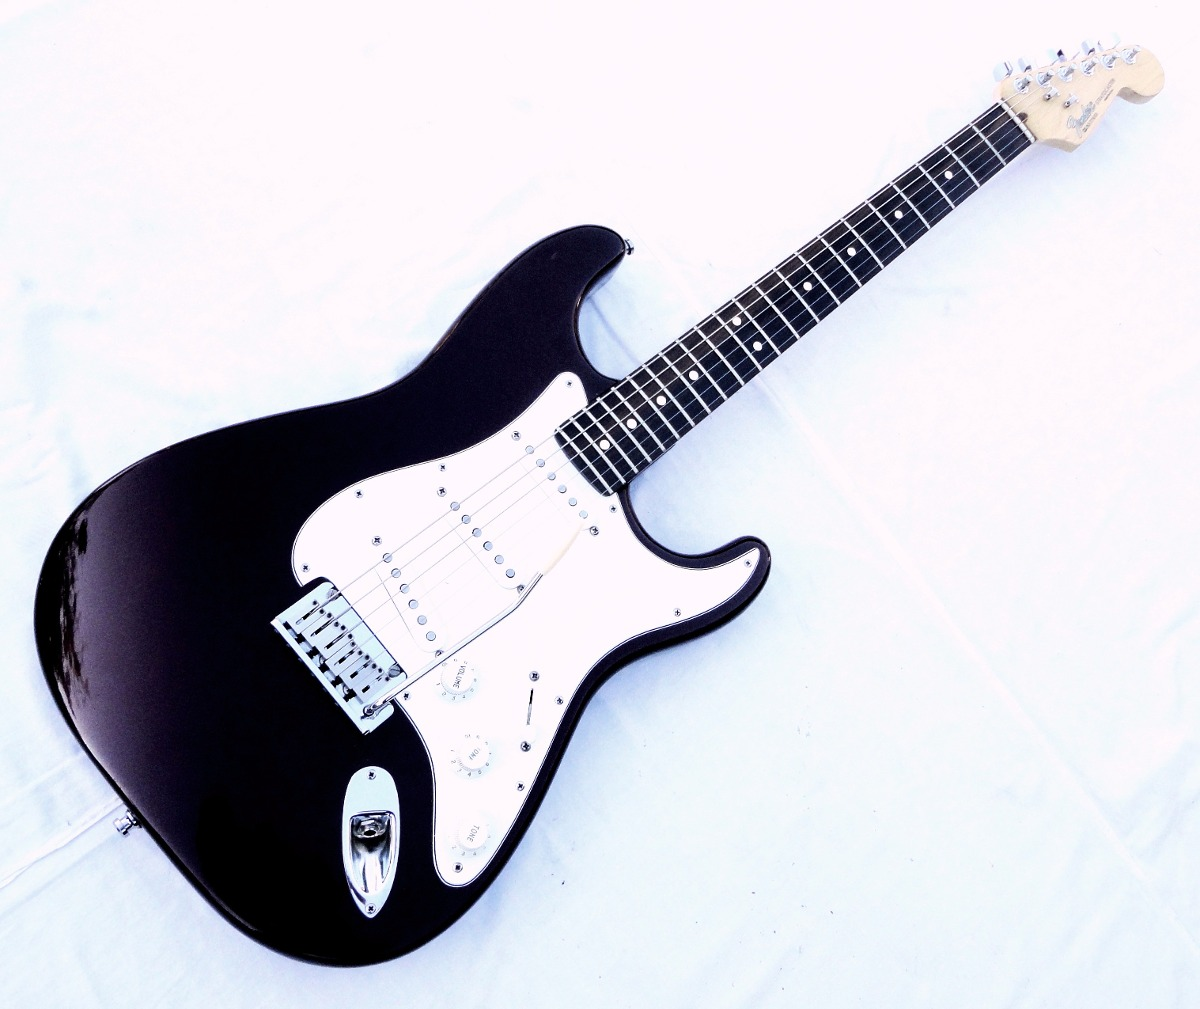
\includegraphics[scale=0.1]{guitarra-electrica-fender-stratocoaster-american-standard-D_NQ_NP_632980-MLM25679231814_062017-F.jpg}\\
En mi caso, un objeto muy simbólico para mí es una guitarra eléctrica, esto porque muestra mi profundo amor por la música y el gran gusto que le tengo a tocar mis canciones favoritas en guitarra (aunque no sepa componer); y específicamente, estea guitarra es igual a la primera que tuve y que sigo usando, le tengo mucho cariño.
\end{frame}

\begin{frame}{Teorema de Morgan \cite{teoremamorgan}}
    El teorema de Morgan se me hizo ciertamente interesante pues ayuda a simplificar expresiones booleanas, y cambiar el operador de disyunción por el de conjunción y viceversa. Si no me equivoco, pertenece a la lógica proposicional y al álgebra booleana.\\
    Me gustó porque, por lo que leí, demuestra también que la conjunción y la disyunción son como las bases de la lógica proposicional, pues de ellos parten los demás conectores lógicos.
\end{frame}

\begin{frame}{Ecuación a resolver}

Ahora vamos a resolver la función \underline{$\frac{3}{4}x+9=15$} (o más bien verificarla).\\
Empecemos por despejar 9, por lo que nos queda de la siguiente manera: \underline{$(\frac{3}{4}x+9)-9=(15)-9$}, y a su vez termina siendo \underline{$\frac{3}{4}x=6$.}
Ahora, si reescribimos la ecuación, nos queda como \underline{$\frac{3x}{4}=6$}, y ahora vamos a despejar el 4 de la siguiente forma: \underline{$4(\frac{3x}{4})=(6)4$}.\\
Después de despejar 4, la ecuación nos queda como \underline{$3x=24$}, y ahora nos toca despejar el 3 de la siguiente forma: \underline{$(3x)/3=(24)/3$}.\\
Una vez despejamos 3, la ecuación queda de la siguiente forma: \underline{$x=8$}. Esto nos dice que el valor de x es 8.
    
\end{frame}

\begin{frame}{Bibliografía}
    \bibliographystyle{plain}
    \bibliography{Bibliografía_ejercicio_1}
\end{frame}

\end{document}